\chapter{Produtos, Atividades e Cronograma}

\section{Estrutura Analítica do Projeto}

\begin{figure}[!htp]
		\centering
		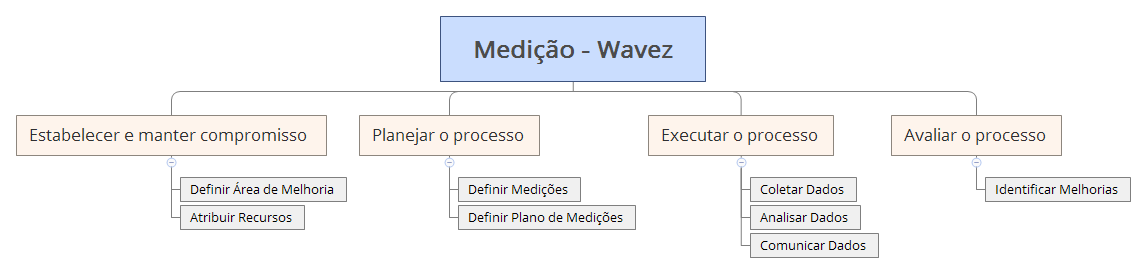
\includegraphics[scale=0.40]{figuras/eap}
		\label{img:processo}
		\caption{Visão geral do Processo de Medição}
\end{figure}

\section{Descrição das Atividades}

\begin{table}[!htpd]
\centering
\caption{\textbf{Estabelecer e manter compromisso com o processo de medição}}
\label{my-label}
\begin{tabular}{|c|c|c|}
\hline
Atividade                & Descrição                                                                                                                                                               & Responsáveis \\ \hline
\begin{tabular}[c]{@{}c@{}} Definir Área \\ de Melhoria\end{tabular} & \begin{tabular}[c]{@{}c@{}}Esta atividade consiste em definir um projeto, bem \\ como a área a ser realizada o processo de medição\\ e em definir o escopo\end{tabular} & Todos        \\ \hline
\begin{tabular}[c]{@{}c@{}} Atribuir \\ Recursos\end{tabular}       & \begin{tabular}[c]{@{}c@{}}Atividade responsável por alocar recursos com \\ competênciapara a execução do processo\end{tabular}                                         & Todos        \\ \hline
\end{tabular}
\end{table}

\begin{table}[!htpd]
\centering
\caption{\textbf{Planejar o processo de medição}}
\label{my-label}
\begin{tabular}{|c|c|c|}
\hline
Atividade                                                           & Descrição                                                                                                                            & Responsáveis \\ \hline
\begin{tabular}[c]{@{}c@{}}Definir \\Medições\end{tabular}                                                  & \begin{tabular}[c]{@{}c@{}}Esta atividade consiste em definir as métricas\\ a serem coletadas durante o processo\end{tabular}        & Todos        \\ \hline
\begin{tabular}[c]{@{}c@{}}Definir Plano\\ de Medições\end{tabular} & \begin{tabular}[c]{@{}c@{}}Esta atividade consiste em estabelecer como será \\ executada a coleta e análise de métricas\end{tabular} & Todos        \\ \hline
\end{tabular}
\end{table}

\begin{table}[!htpd]
\centering
\caption{\textbf{Executar o processo de medição}}
\label{my-label}
\begin{tabular}{|c|c|c|}
\hline
Atividade                                                       & Descrição                                                                                                                                                                               & Responsáveis \\ \hline
\begin{tabular}[c]{@{}c@{}}Coletar \\ Dados\end{tabular}        & \begin{tabular}[c]{@{}c@{}}Atividade responsável pela coleta de métricas\\  previamente definidas\end{tabular}                                                                          & Todos        \\ \hline
\begin{tabular}[c]{@{}c@{}}Analisar\\ Dados\end{tabular}        & \begin{tabular}[c]{@{}c@{}}Esta atividade consiste na análise das  métricas \\ coletadas, a fim de que obtenha-se um \\ entendimento do impacto dessas métricas no projeto\end{tabular} & Todos        \\ \hline
\begin{tabular}[c]{@{}c@{}}Comunicar\\  Resultados\end{tabular} & \begin{tabular}[c]{@{}c@{}}Esta atividade consiste na descrição\\  da análise feita sobre as métricas\end{tabular}                                                                      & Todos        \\ \hline
\end{tabular}
\end{table}

\begin{table}[!htpd]
\centering
\caption{\textbf{Avaliar o processo de medição}}
\label{my-label}
\begin{tabular}{|c|c|c|}
\hline
Atividade                                                        & Descrição                                                                                                                                       & Responsáveis \\ \hline
\begin{tabular}[c]{@{}c@{}}Identificar\\  Melhorias\end{tabular} & \begin{tabular}[c]{@{}c@{}}Atividade responsável por identificar possíveis \\ melhorias a serem feitas dada a análise das métricas\end{tabular} & Todos        \\ \hline
\end{tabular}
\end{table}
